\documentclass[a4paper]{report}
\pagestyle{headings}
\usepackage{hyperref}
\usepackage{listings}
\usepackage{graphicx}
\usepackage{subfiles}
\usepackage{multirow}
\usepackage[table,xcdraw]{xcolor}
\lstset{numbers=right}
\lstset{breaklines}
\title{Lab Report for Software Engineering course \newline
 Lab 6: Demand Documentation}
\author{Wang, Chen\qquad Liu, Jiaxing\qquad Huang, Jiani\qquad Tang, Xinyue \\
16307110064\qquad17302010049\qquad 17302010063\qquad 16307110476 \\
School of Software\\
Fudan University
}
\date{\today}
\bibliographystyle{plain}
\begin{document}
\maketitle

\tableofcontents
\chapter{Revision History of the demand documentation}

\begin{tabular}{|c|c|c|c|} 
\hline 
Modifier&Modify Time&Approver&Modified Chapter\\
\hline  
Huang Jiani&2019-6-19&All&Refined Function Requirements\\
\hline 
\end{tabular}

\chapter{Project Outline}
\section{Background information of the project}

\section{Overview of the features of the project}

\section{Module division of the project}

\section{User characteristics of the project}

\section{Runtime environment}

\section{Conditions and restrictions}

\chapter{Feature Demands}

% Huang 2019-06-18 below
\section{Refined function requirements}
According to the interview record of the lab assigner, t the whole system should satisfy the requirements in the following perspectives:
\subsection{Administration access Authorization}
\begin{enumerate}
\item Any shop assistant must first get authorized administration access of the system before he conducts all the normal routines including signing up, logging in, matching drinks, getting drink descriptions and ordering. 
\item Anyone except shop assistants is unauthorized to the administration access.
\item To get the authorized administration access, the shop assistant must do XXXXXX.
\end{enumerate}

\subsection{Signing up}
\begin{enumerate}
\item Any shop assistant can use the unique username and password to sign up.
\item The username will be persistently recorded in the user.csv (?) after the shop assistant signs up.
\item The username must start with \textbf{starbb\_};
\item The username can consist of \textbf{letters}, \textbf{numbers} and \textbf{underline}, excluding any other symbols;
\item The username should have a length greater than or equal to 8 and less than 50.
\item The password can consist of \textbf{letters}, \textbf{numbers} and \textbf{\_}, excluding any other symbols;
\item The password must consist of all the three types, i.e. \textbf{letters}, \textbf{numbers} and \textbf{\_}, excluding any other symbols;
\item The password should have a length greater than or equal to 8 and less than 100.
\end{enumerate}

\subsection{Logging in}
\begin{enumerate}
\item Only if the shop assistant logs in successfully can he do the other normal routines including matching drinks, getting drink descriptions and ordering.
\item The shop assistant will log in successfully if and only if the username and password are matched.
\item The login status will be recorded after the shop assistant logs in successfully.
\item If the shop assistant fails to log in, the system will throw a runtime exception to prompt the failed login.
\item If the shop assistant fails to log in because of wrong password, the system will prompt \textbf{Username or password error};
\item If the shop assistant fails to log in, he will not allowed to conduct any other operations.
\end{enumerate}

\subsection{Matching drinks}

\begin{enumerate}
\item The shop assistant can get different drinks considering different cup sizes and different kinds and numbers of ingredients.
\end{enumerate}


\subsection{Obtaining drink descriptions}
\begin{enumerate}
\item The shop assistant can obtain and check different descriptions of drinks.
\item The customer can obtain and check different descriptions of drinks.
\end{enumerate}

\subsection{Order charge calculation}
\begin{enumerate}
\item The shop assistant can order according to the verbal instructions of the customer.
\item The shop assistant can calculate the order charge including the original price, discount and the total discount charge.
\item The customer can check the order charge including the original price, discount and the total discount charge.
\end{enumerate}

\subsection{Drinks supported}
\begin{enumerate}
\item The default drinks include coffee and tea.
\item The default coffee includes Espresso and Cappuccino.
\item The default tea includes GreenTea and RedTea.
\item Different stores can customize their own drinks of local characteristics.
\item Every drink should have attributes of its name, price and description(?).

\end{enumerate}

\subsection{Ingredients supported}
\begin{enumerate}
\item The default ingredients include milk, chocolate, cream and sugar.
\item The prices of ingredients can be fixed by the maintenance personnel.
\item Different kinds and numbers of Ingredients can be added .
\end{enumerate}

\subsection{Cup size supported}
\begin{enumerate}
\item There are totally three kinds of cup size : large, middle and small.
\end{enumerate}

\subsection{Discount supported}
\begin{enumerate}
\item There are three categories of discount strategies in total : Double eleven, Full count and Combination.
\item Combination strategy has four concrete strategies.
\item The concrete strategies can have superposition.
\item Different categories of discount strategies cannot have superposition.
\begin{enumerate}
\item Order including both tea and coffee will have 15\% discount.
\item 2 cups of Large-cup Espresso will have 20\% off discount.
\item Buying three cups of tea will send one for free.
\item Cappuccino second half price.
\end{enumerate}
\item Full count: All drinks full 100 minus 30
\item Double Eleven: All drinks 50\% off.
\end{enumerate}

\subsection{Language switch}
\begin{enumerate}
\item The system language can be switched to the official language of different countries and regions.
\item The language switch should cover everywhere customers can see and check.
\item The default supported languages are Chinese and English.
\end{enumerate}

\subsection{Currency switch}
\begin{enumerate}
\item The currency switch will not consider exchange rate fluctuations.
\item The currency should be switched according to different countries and regions.
\item The default supported currencies are Chinese Yuan, Hong Kong dollar and US dollar.
\end{enumerate}

\subsection{Price fix}
\begin{enumerate}
\item The maintenance personnel can fix the prices of all the items.
\end{enumerate}

\subsection{Configuration and Maintenance}
\begin{enumerate}
\item The maintenance personnel can configure and maintain all the settings including drinks, ingredients, cup-size, discount, language, currency and price-fixing.

\end{enumerate}

\subsection{log information supported}
\begin{enumerate}
\item The system must provide log information for the maintenance personnel.
\item The log information must include records of order errors and successful order cases.
\end{enumerate}

\section{Detailed description of refined function requirements}

\subsection{Scenario analysis and modeling}
We apply the use case diagram to the scenario analysis and modeling procedure. As the diagram shows, there are two actors including customers and shop assistants and the online  system in the whole interaction. Ordering and register are the  two main use cases. Several sub use cases of ordering like beverage information checking, beverage matching and beverage price calculating. And All these use cases include the smaller login user case.
\begin{figure}
  \centering
  \includegraphics[scale=0.44]{figure1.jpg}
  \caption{Overall Use-case Diagram}\label{2}
\end{figure}

\subsubsection{Use case 1: Ordering}
In this use-case, we apply the swim lane diagram to concisely describe the relationship between users and the system.
\begin{itemize}
\item \textbf{Use-case name:} ordering
\item \textbf{Actors:} customers and shop assistants
\item \textbf{Target:} The shop assistant can complete the order-making process according to the verbal instruction of customers.
\item \textbf{Precondition:} The shop assistant has registered before. 
\item \textbf{Triggering condition:} There is a customer waiting to order in the store.
\item \textbf{Main scene:} After the shop assistant logs in the system successfully, he/she waits for the verbal instructions of the customer. After the customer tells him/her the wanted cup-size, ingredients and kind of  beverages, the shop assistant can make an ordering, and tells the customer the total price, discounted price and discount information of the order. After the customer has paid the charge, the order is finished and the system will be waiting for another order.
\item \textbf{Abnormal scenes:}
\begin{enumerate}
\item  \textbf{Login failure:} If the shop assistant enters wrong username or password, he can get the chance to enter again until he finally enters the correct username and password and logs in the system. 

\item \textbf{Order failure:} If the order process is interrupted due to the internet or other hardware break, the order process will return back to the calculating procedure after recovery.
\end{enumerate}
\item \textbf{Frequency:} The ordering use-case will be continuing 24 hours a day only if there is a customer waiting to order.
\end{itemize}

\subsubsection{Use case 2: Register}
In the ordering user-case, we apply the activity diagram to describe the whole process. 
 \begin{itemize}
\item \textbf{Use-case name:}  registering
\item \textbf{Actors:} shop assistants
\item \textbf{Target:} The shop assistant can complete the registering process.
\item \textbf{Precondition:} 
\begin{enumerate}
\item The server of the system is running normally.
\item The shop assistant has gained the access authorization before.
\end{enumerate}
\item \textbf{Triggering condition:} None
\item \textbf{Main scene:} After the shop assistant gains the access authorization successfully, he can enter the system to choose login or register. After he enters the valid username and password, he can use them to login and make orders.
\item \textbf{Abnormal scenes:} 
\begin{enumerate}
\item  \textbf{Password invalid:} If the shop assistant enters invalid password, the system will prompt corresponding message and let the user enter again untill he enters the valid password.
\item \textbf{Username invalid:} If the shop assistant enters invalid username, the system will prompt corresponding message and let the user enter again until he enters the valid username.
\end{enumerate}
\item \textbf{Frequency:}  Relatively low, since only when there is new and unregistered shop assistant will it be triggered. However, the register use-case should be available 24 hours a day. 
\end{itemize}

\subsection{Class analysis and modeling}
\subsubsection{Analysis class extraction}
\begin{itemize}
\item User
\item AccountService
\item OrderItem
\item Order
\item PaymentInfo
\item OrderService
\item MarketingStrategy
\item DoubleElevenStrategy
\item FullDiscountStrategy
\item CombinationDiscountStrategy
\item LanguageService
\item MenuService
\end{itemize}

\subsubsection{Function of classes}
\begin{itemize}
\item \textbf{User :} The entity class represents shop assistants. There are two attributes: name and password.
\item \textbf{AccountService :} The service class is charge of the login, signup, status-checking, name-checking and password-checking of users.
\item \textbf{OrderItem :} The entity class represents beverages. There are three attributes: name, size and ingredients. Also, it has a public method to calculate the price according to its size and ingredients.
\item \textbf{Order :} The DTO class is used to transfer data from server to client end. There are three attributes: id, currency and orderItems. Also, it has a public method to calculate the total charge of the order. 
\item \textbf{PaymentInfo :} The class is composed of all the return information of the order, including price, discount, discountPrice and messages.
\item \textbf{OrderService :} The service class includes one attribute strategies and one public method pay.
\item \textbf{MarketingStrategy :} The strategy class include one public method getDiscount. And all the  sub strategy classes including  DoubleElevenStrategy, FullDiscountStrategy and CombinationDiscountStrategy inherit it.
\item \textbf{LanguageService :} The service class has one public method updateLanguage.
\item \textbf{MenuService :} The service class has one public method getPrice according to different countries and regions.
\end{itemize}
\subsubsection{Relationship between classes}
As the UML diagram shows, the relationships in this system can be divided into three kinds: inheritance, composition and dependency.
\begin{figure}
  \centering
  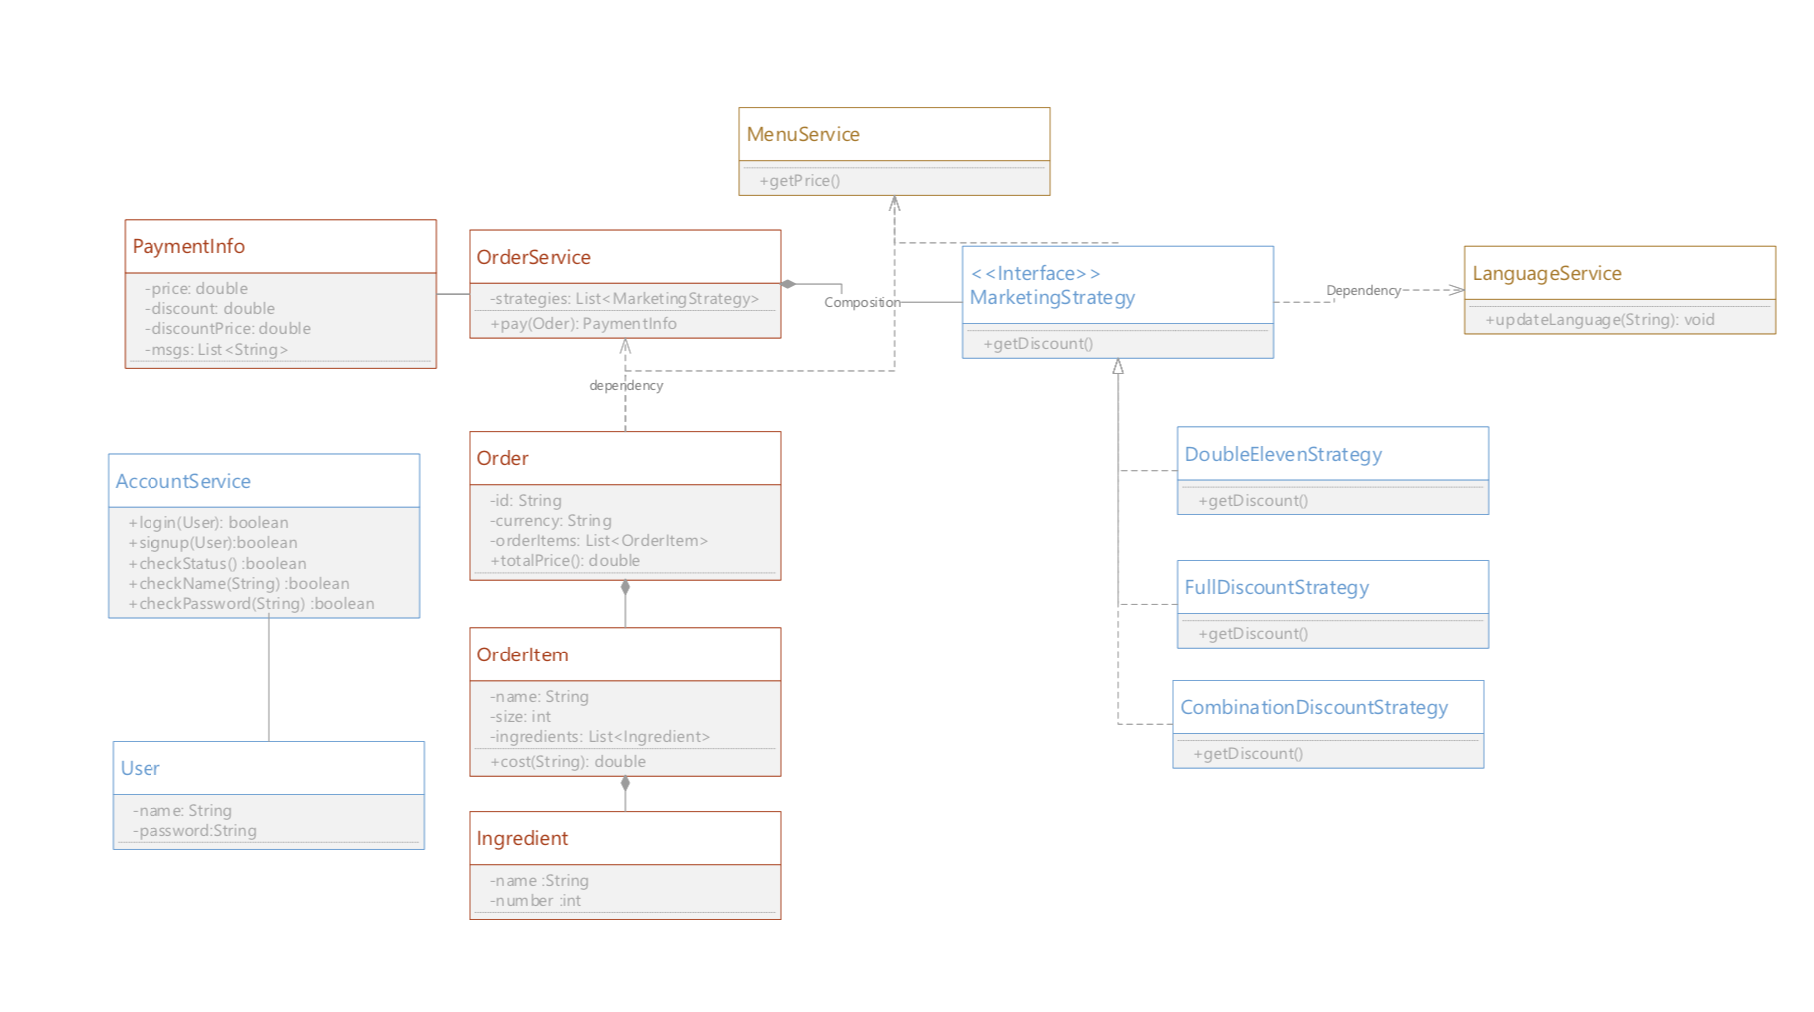
\includegraphics[scale=0.44]{figure4.jpg}
  \caption{Overall UML Class Diagram}\label{2}
\end{figure}
\subsection{Data Flow analysis and modeling}
\subsubsection{level 0:}
\subsubsection{level 1:}
\subsubsection{level 2:}

\subsection{Behavior analysis and modeling}


\chapter{Performance Demands}

\section{Massive end user support}
\subsection{Detailed Description}
There will be about 200 stores using this system at the same time. And the scale will be about 1000 people per day. The people using this system includes XXX.
\subsection{Proposed measures}
Since the system will be built on several servers, the strategies like load balancing can be used to handle the big amount of customers.

\section{Stability over long period of time}
\subsection{Detailed Description}
Since the store will be open 24 hours a day, the system must be running all the time and at least maintained evert half a year.
\subsection{Proposed measures}
This requires that the system should not stop or exit by accident at any time. We should handle all the possible accidents and catch the exceptions.

\chapter{Appendix}
\section{Demand interview outline}
\subsection{Constraints (5 minutes)}
\begin{enumerate}
\item What is the number of servers? 
\item Is there a regulation or limitation on the system running server-side operating system? 
\item What are the rules or restrictions for the client device operating system (in the store)? 
\item Is the salesperson's computer equipped with a screen for the customers?
\item Are there still any other special hardware conditions (supplementary)? 
\item Does the company have specific legal restrictions? 
\item The development time and delivery time points given? 
\item Is there an intermediate time frame when partial project need to be examined?
\end{enumerate}
 \subsection{Performance requirements (5 minutes)}
 \begin{enumerate}
\item Is 1,000 person/day referring to the salesperson or the customer (personal * month) ? What is the upper limit? 
\item What is the number of the stores in the description ``Support the usage of massive stores concurrently''?  What is the average number of orders in the store? And what about the peak order number? 
\item Order response time? 
\item ``Long-running and stable support system ": the requirements for a client front end and user-friendliness, cannot be unable to play due to any reason except network or hardware issues, cannot crash under massive clients, cannot have severe bug after online
\end{enumerate}
\subsection{Functional requirements(15 minutes)}
\begin{enumerate}
\item Drinks, ingredients, cups in the beverage store supported by the system 
\item Superposition and mutual exclusion of offers 
\item Language, currency, pricing 
\item Register \& log in 
\item Order versus Associate / independent with drinks, price, and description?
\item What the customer sees: the information returned in the order content and paymentInfo , including the beverage, original price, discounted price, discount information (whether it is necessary to specify the description of each beverage) 
\item How the salesperson gets permission 
\item Log information provided by the system 
\item Process confirmation again
\end{enumerate}
\subsection{Possible modification of the code}
\begin{enumerate}
\item Increase currency dollar 
\item Salesperson access 
\item Offer modification 
\item View all aspects of drinks and ingredients (cup type, price) individual customer / salesperson interface 
\end{enumerate}
\subsection{About the requirements document }
\begin{enumerate}
\item ``Give a corresponding map and explanation for each demand"
\end{enumerate}
\section{Organized interview records}
\section{Code change logs in response of new demands}

% Huang 2019-06-18 above



\begin{thebibliography}{A}


\bibitem{1}
Wikipedia contributors. (2019, March 22). JUnit. In \emph{Wikipedia, The Free Encyclopedia}. Retrieved 14:53, April 1, 2019, from \url{https://en.wikipedia.org/w/index.php?title=JUnit&oldid=888928403}
\end{thebibliography}
\end{document} 